\documentclass[aspectratio=43]{beamer}
\usepackage[utf8]{inputenc}
\usepackage[T1]{fontenc}
\usepackage[brazil]{babel}
\usepackage{amsmath, amssymb}
\usepackage{booktabs}
\usepackage{graphicx}

% Tema limpo idêntico ao padrão clássico de COS360
\usetheme{Madrid}
\usecolortheme{whale}
\setbeamertemplate{navigation symbols}{}

\title[Otimização de Portfólio via Barreira Logarítmica]{Otimização Convexa de Portfólio via Método de Barreira Logarítmica}
\subtitle{Aplicação ao Agronegócio Brasileiro com Ponderação Climática}
\author{João Chamarelli}
\institute[UFRJ / COS360]{Disciplina: COS360 -- Otimização \\ Universidade Federal do Rio de Janeiro}
\date{Novembro de 2026}

\begin{document}

%---------------------------------------------------------
% Slide 1: Capa
%---------------------------------------------------------
\begin{frame}
  \titlepage
\end{frame}

%---------------------------------------------------------
% Slide 2: Introdução e Histórico
%---------------------------------------------------------
\begin{frame}{Introdução e Motivação}
  \begin{itemize}
    \item \textbf{Markowitz (1952):} \emph{trade-off} média-variância (QP convexo com $w \ge 0$).
    \item \textbf{Barreira Logarítmica:} Fiacco \& McCormick (1968); pontos interiores com Karmarkar (1984) e Nesterov \& Nemirovski (1994); algoritmo de Boyd \& Vandenberghe (2004, cap.~11).
    \item \textbf{Usos atuais:} núcleo de \emph{solvers} (MOSEK, Gurobi, CPLEX) e gestão quantitativa de carteiras.
    \item \textbf{Aplicação:} cadeia ampliada do agro na B3, setor sensível ao clima.
  \end{itemize}
\end{frame}

%---------------------------------------------------------
% Slide 3: Instância e Motivação
%---------------------------------------------------------
\begin{frame}{Problema e Instância de Dados}
  \begin{itemize}
    \item \textbf{Objetivo:} Alocar pesos $w \in \mathbb{R}^N$ entre $N = 20$ ações da cadeia ampliada do agro na B3, balanceando retorno esperado e variância.
    \item \textbf{Estimação:} Janela histórica mensal de jan/2015 a dez/2024 ($T = 120$ meses).
    \item \textbf{Momentos com pesos de cenário $p_t \ge 0$ ($\sum_{t=1}^T p_t = 1$):}
    \[
      \mu = 12\,\bar{r} = 12\sum_{t=1}^T p_t r_t, \qquad
      \Sigma = 12\sum_{t=1}^T p_t (r_t - \bar{r})(r_t - \bar{r})^\top
    \]
    \item \textbf{Duas instâncias para teste de sensibilidade:}
    \begin{enumerate}
      \item \textbf{Base:} $p_t = 1/T$ (todos os meses com peso igual).
      \item \textbf{Climático (Kernel 11D):} $p_t \propto \exp\!\left(-\frac{\|z_{t-8} - z_{T-8}\|_2^2}{2\sigma^2}\right)$ ($\sigma = 2{,}0$) sobre 11 variáveis climáticas (temp., chuva e ONI), comparando com $z_{T-8}$ (abr/2024).
    \end{enumerate}
  \end{itemize}
\end{frame}

%---------------------------------------------------------
% Slide 4: Formulação Matemática, Convexidade e Premissas
%---------------------------------------------------------
\begin{frame}{Formulação Matemática, Convexidade e Premissas}
  Para aversão ao risco $\gamma = 5$:
  \[
  \begin{aligned}
    \min_{w \in \mathbb{R}^N}\quad & f(w) = \frac{\gamma}{2}\, w^\top \Sigma\, w \;-\; \mu^\top w \\
    \text{s.a.}\quad & \mathbf{1}^\top w = 1 \quad (\text{orçamento}), \qquad w_i \ge 0,\; i = 1, \dots, N \quad (\text{sem venda a desc.})
  \end{aligned}
  \]

  \begin{block}{Convexidade Estrita e Unicidade}
    Como $v^\top \Sigma v = 12 \sum_{t=1}^T p_t ((r_t - \bar{r})^\top v)^2 \ge 0$ e $\lambda_{\min}(\Sigma) = 0{,}0387 > 0$, temos $\nabla^2 f(w) = \gamma\Sigma \succ 0$ no simplex $\Delta_N$: o problema é \textbf{estritamente convexo}, logo toda solução KKT é o \textbf{mínimo global único}.
  \end{block}

  \scriptsize
  \textbf{Aproximações e premissas:} $(\mu,\Sigma)$ estimados são tratados como verdadeiros; anualização $\times 12$ supõe meses independentes; carteira estática (decisão em dez/2024), sem custos de transação ou restrição de liquidez; $\gamma = 5$ escolhido (sensibilidade no Slide~12).
\end{frame}

%---------------------------------------------------------
% Slide 5: Condições de KKT e Solução Fechada
%---------------------------------------------------------
\begin{frame}{Condições de KKT e Benchmark Analítico}
  \textbf{Lagrangeano:}
  $\mathcal{L}(w,\nu,\lambda) = \frac{\gamma}{2}w^\top\Sigma w - \mu^\top w + \nu(\mathbf{1}^\top w - 1) - \lambda^\top w$

  \vspace{0.15cm}
  \begin{columns}[T]
    \begin{column}{0.48\textwidth}
      \textbf{Condições KKT:}
      \begin{itemize}
        \item $\gamma\Sigma w^* - \mu + \nu^*\mathbf{1} - \lambda^* = 0$
        \item $\mathbf{1}^\top w^* = 1,\; w^* \ge 0$
        \item $\lambda^* \ge 0$
        \item $\lambda_i^* w_i^* = 0 \;\; \forall i$ (folga compl.)
      \end{itemize}
    \end{column}
    \begin{column}{0.50\textwidth}
      \textbf{Forma fechada sem $w \ge 0$ ($\lambda = 0$):}
      \[
        w^* = \frac{1}{\gamma}\Sigma^{-1}(\mu - \nu^*\mathbf{1}), \qquad
        \nu^* = \frac{\mathbf{1}^\top\Sigma^{-1}\mu - \gamma}{\mathbf{1}^\top\Sigma^{-1}\mathbf{1}}
      \]
      \small
      \begin{itemize}
        \item Vende \textbf{8 de 20 ativos} a descoberto (até $-23{,}3\%$).
        \item Impor $w \ge 0$ muda todo o conjunto ativo: a barreira zera \textbf{12 ativos} (incluindo \texttt{RAPT4}, de $+27{,}5\%$ para $0\%$), e $\lambda_i^* > 0$ atua como preço-sombra.
      \end{itemize}
    \end{column}
  \end{columns}
\end{frame}

%---------------------------------------------------------
% Slide 6: Método de Barreira Logarítmica
%---------------------------------------------------------
\begin{frame}{Método de Barreira Logarítmica}
  \textbf{1. Eliminação da igualdade $\mathbf{1}^\top w = 1$:} parametrizamos $x \in \mathbb{R}^{N-1}$ com
  \[
    w(x) = A x + e_N, \qquad
    A = \begin{bmatrix} I_{N-1} \\ -\mathbf{1}_{N-1}^\top \end{bmatrix}, \quad
    e_N = \begin{bmatrix} 0 \\ \vdots \\ 0 \\ 1 \end{bmatrix}
    \implies \mathbf{1}^\top w(x) = 1 \;\; \forall x.
  \]

  \textbf{2. Substituição de $w \ge 0$ pela barreira ($t > 0$):}
  \[
    \phi_t(x) = \frac{\gamma}{2} w(x)^\top \Sigma w(x) - \mu^\top w(x) - \frac{1}{t}\sum_{i=1}^N \log w_i(x)
  \]

  \textbf{3. Derivadas analíticas (regra da cadeia):}
  \small
  \begin{align*}
    \nabla \phi_t(x) &= A^\top\!\left(\gamma\Sigma w(x) - \mu - \frac{1}{t}\, w(x)^{-1}\right) \in \mathbb{R}^{N-1} \\
    \nabla^2 \phi_t(x) &= A^\top\!\left(\gamma\Sigma + \frac{1}{t}\,\mathrm{diag}\big(w(x)^{-2}\big)\right)A \in \mathbb{R}^{(N-1)\times(N-1)}
  \end{align*}
\end{frame}

%---------------------------------------------------------
% Slide 7: Caminho Central, Dualidade e Gap N/t
%---------------------------------------------------------
\begin{frame}{Caminho Central, Gap de Dualidade e Multiplicadores}
  \begin{itemize}
    \item \textbf{Algoritmo:} Para $t \in \{10^1, 10^2, 10^3, 10^4, 10^5, 10^6\}$, minimizamos $\phi_t(x)$ sem restrições usando \emph{warm-start} do estágio anterior.
    \item \textbf{Recuperação gratuita dos multiplicadores KKT:} No mínimo $x^*(t)$ ($\nabla\phi_t = 0$), definimos
    \[
      \hat{\lambda}_i(t) = \frac{1}{t\, w_i(t)} > 0.
    \]
    Como $\mathcal{N}(A^\top) = \mathrm{span}\{\mathbf{1}\}$, existe $\hat{\nu}(t)$ satisfazendo exatamente a estacionariedade KKT.
    \item \textbf{Limitante teórico do gap de dualidade:}
    \[
      f(w(t)) - f^* \;\le\; \sum_{i=1}^N \hat{\lambda}_i(t)\, w_i(t) \;=\; \frac{N}{t}.
    \]
    Para $N = 20$ e $t = 10^6$, o erro na função objetivo é no máximo $2 \times 10^{-5}$.
  \end{itemize}
\end{frame}

%---------------------------------------------------------
% Slide 8: Por que Newton na Barreira?
%---------------------------------------------------------
\begin{frame}{Por que Newton na Barreira? Subproblemas Irrestritos}
  \begin{table}
    \centering
    \scriptsize
    \begin{tabular}{@{}llll@{}}
      \toprule
      \textbf{Método} & \textbf{Direção $d_k$} & \textbf{Taxa Teórica} & \textbf{Custo/Passo} \\
      \midrule
      Gradiente & $-\nabla\phi_t(x_k)$ & Linear ($\frac{\kappa-1}{\kappa+1}$, quadrática, busca exata) & $O(N^2)$ \\
      BFGS & $-B_k\nabla\phi_t(x_k)$ (posto-2) & Superlinear & $O(N^2)$ \\
      Newton & $-[\nabla^2\phi_t(x_k)]^{-1}\nabla\phi_t(x_k)$ & Quadrática & $O(N^3)$ \\
      \bottomrule
    \end{tabular}
  \end{table}

  \vspace{0.15cm}
  \begin{block}{Busca Linear de Armijo com Salvaguarda de Domínio}
    Partindo de $\alpha = 1$ ($\beta = 0{,}5$, $c = 10^{-4}$):
    \begin{enumerate}
      \item \textbf{Salvaguarda:} enquanto $\min_i w_i(x_k + \alpha d_k) \le 0$, faça $\alpha \leftarrow \beta\alpha$ (permanece no domínio de $\log w_i$).
      \item \textbf{Armijo:} enquanto $\phi_t(x_k + \alpha d_k) > \phi_t(x_k) + c\,\alpha\,\nabla\phi_t(x_k)^\top d_k$, faça $\alpha \leftarrow \beta\alpha$.
    \end{enumerate}
  \end{block}
\end{frame}

%---------------------------------------------------------
% Slide 9: Resultado Principal - Convergência e Condicionamento
%---------------------------------------------------------
\begin{frame}{Resultados: Convergência e Mau Condicionamento}
  \begin{table}
    \centering
    \small
    \begin{tabular}{@{}rrrrrrr@{}}
      \toprule
      \textbf{Estágio} & \textbf{$t$} & \textbf{Gap $N/t$} & \textbf{$\kappa(\nabla^2\phi_t)$} & \textbf{Newton} & \textbf{BFGS} & \textbf{Gradiente} \\
      \midrule
      1 & $10^1$ & $2{,}0\times 10^0$ & $22{,}8$ & \textbf{3} & 73 & 125 \\
      2 & $10^2$ & $2{,}0\times 10^{-1}$ & $70{,}0$ & \textbf{5} & 28 & 314 \\
      3 & $10^3$ & $2{,}0\times 10^{-2}$ & $130{,}5$ & \textbf{6} & 44 & 696 \\
      4 & $10^4$ & $2{,}0\times 10^{-3}$ & $1.103{,}3$ & \textbf{7} & 35 & 4.307 \\
      5 & $10^5$ & $2{,}0\times 10^{-4}$ & $11.741{,}8$ & \textbf{7} & 55 & 20.000 (lim.) \\
      6 & $10^6$ & $2{,}0\times 10^{-5}$ & $118.397{,}9$ & \textbf{8} & 50 & 20.000 (lim.) \\
      \midrule
      \textbf{Total} & -- & -- & -- & \textbf{36} & \textbf{285} & \textbf{45.442+} \\
      \bottomrule
    \end{tabular}
  \end{table}

  \small
  \begin{itemize}
    \item \textbf{Por que Newton é o método natural da barreira?} A partir de $t = 10^3$, ativos zerados ($w_i^* = 0, \lambda_i^* > 0$) têm $w_i(t) \approx \frac{1}{t\lambda_i^*} \implies \kappa(\nabla^2\phi_t) = O(t)$ assintoticamente ($\sim 10\times$/estágio), inviabilizando 1ª ordem.
    \item \textbf{Validação:} $\|w_{\text{Newton}} - w_{\text{SLSQP}}\|_\infty = 2{,}25 \times 10^{-4}$; resíduo KKT $= 2{,}04 \times 10^{-9}$; $\max_i |\hat{\lambda}_i w_i| = 10^{-6}$.
  \end{itemize}
\end{frame}

%---------------------------------------------------------
% Slide 10: Gráfico de Convergência
%---------------------------------------------------------
\begin{frame}{Convergência Interna e Explosão de $\kappa(\nabla^2\phi_t)$}
  \begin{figure}
    \centering
    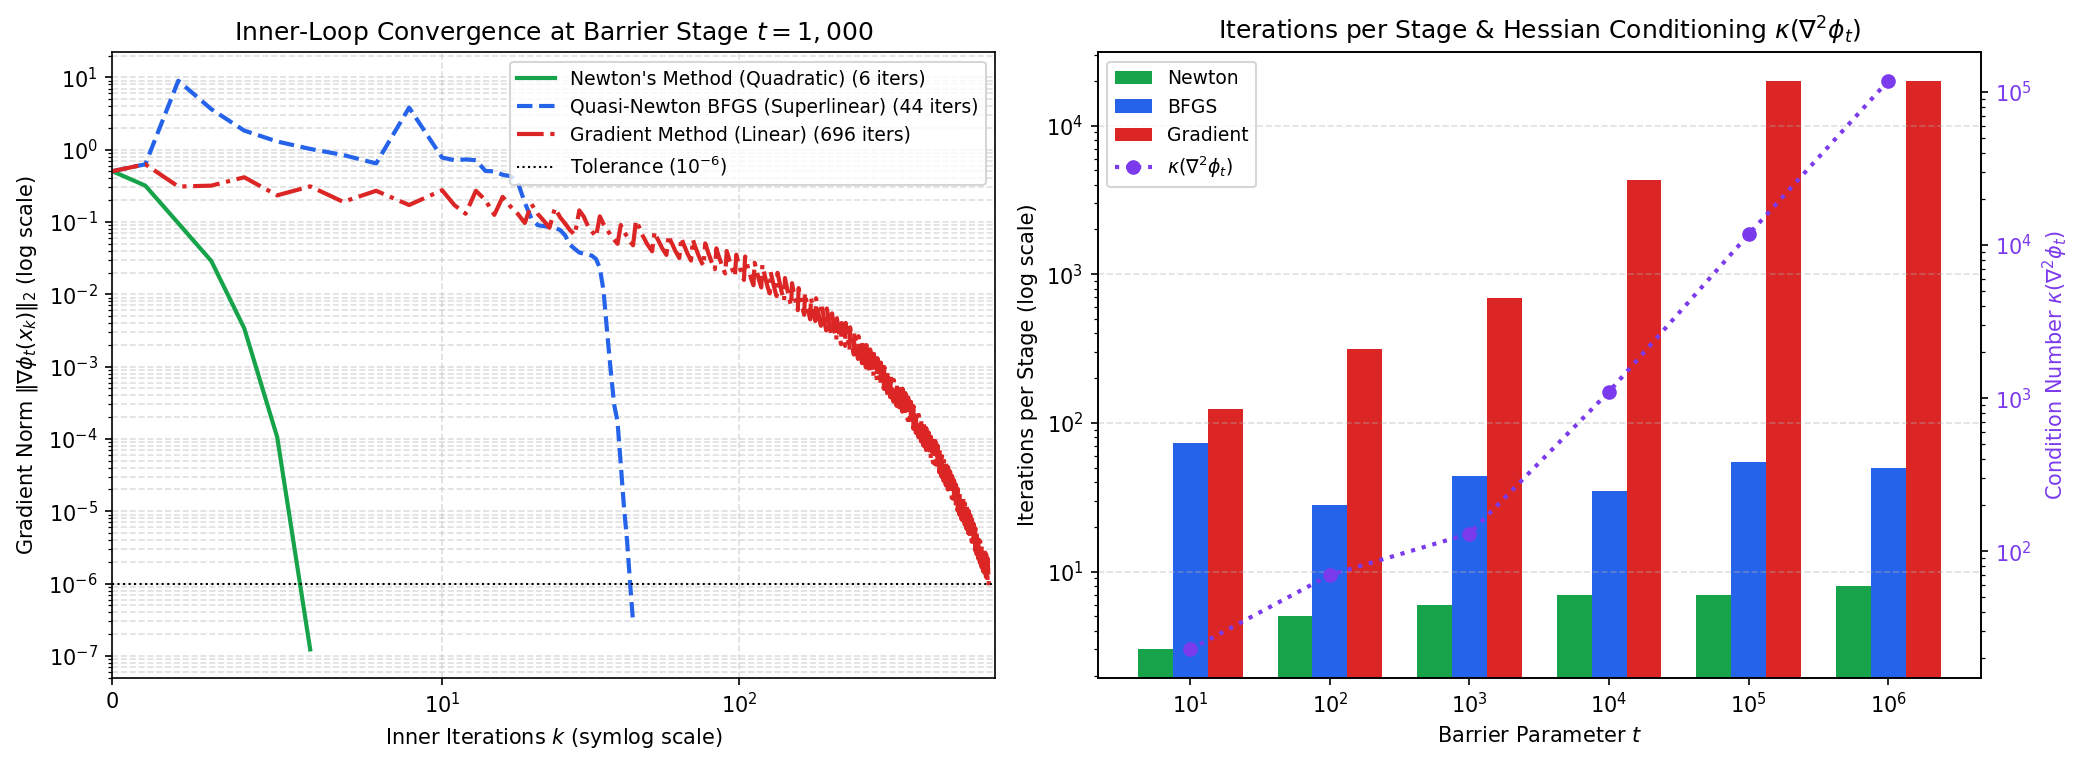
\includegraphics[width=\textwidth, height=0.75\textheight, keepaspectratio]{outputs/fig2_convergence_comparison.png}
  \end{figure}
\end{frame}

%---------------------------------------------------------
% Slide 11: Solução Primal-Dual e Sensibilidade a p_t
%---------------------------------------------------------
\begin{frame}{Esparsidade KKT e Sensibilidade aos Pesos $p_t$}
  \begin{figure}
    \centering
    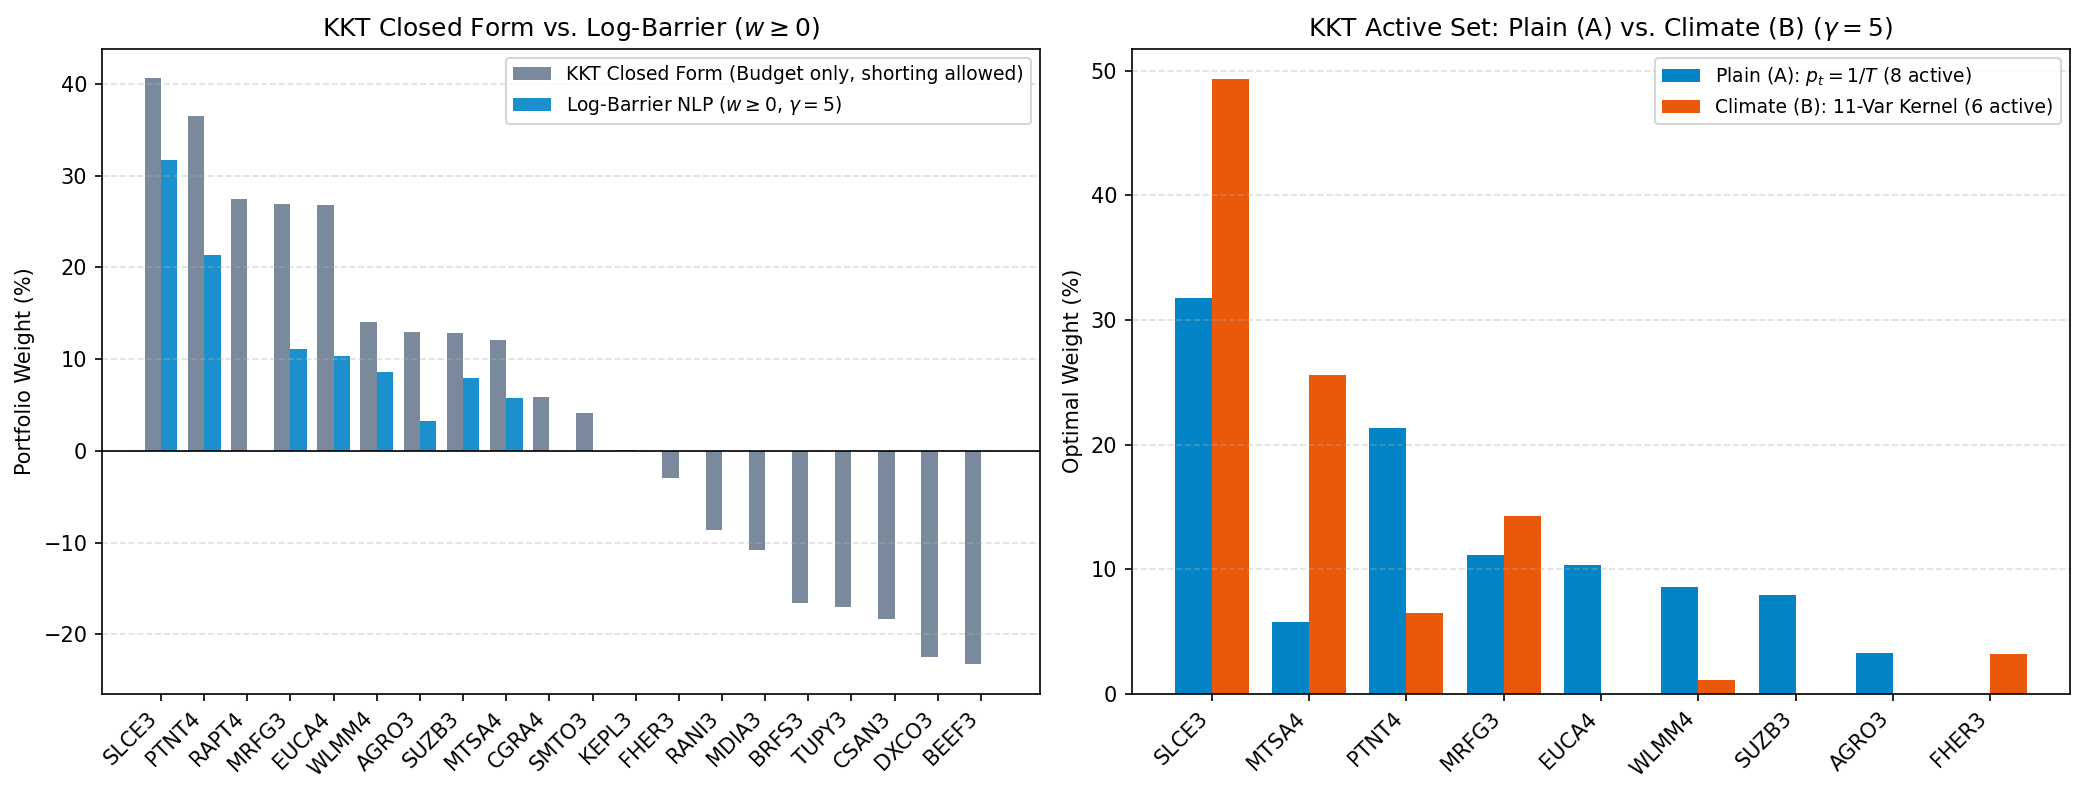
\includegraphics[width=\textwidth, height=0.68\textheight, keepaspectratio]{outputs/fig1_kkt_vs_barrier_weights.png}
  \end{figure}
  \small
  \begin{itemize}
    \item Sem heurística de corte: $w \ge 0$ e $\lambda_i w_i = 0$ zeram $12\text{--}14$ ativos (na ordem de $10^{-6}$), deixando \textbf{8 ativos} (Base) e \textbf{6 ativos} (Clima) com peso $> 0{,}5\%$.
  \end{itemize}
\end{frame}

%---------------------------------------------------------
% Slide 12: Extra - Fronteira Paramétrica e Backtest (2025)
%---------------------------------------------------------
\begin{frame}{Extra: Varredura Paramétrica ($\gamma$) e Backtest (2025)}
  \begin{columns}[T]
    \begin{column}{0.49\textwidth}
      \begin{figure}
        \centering
        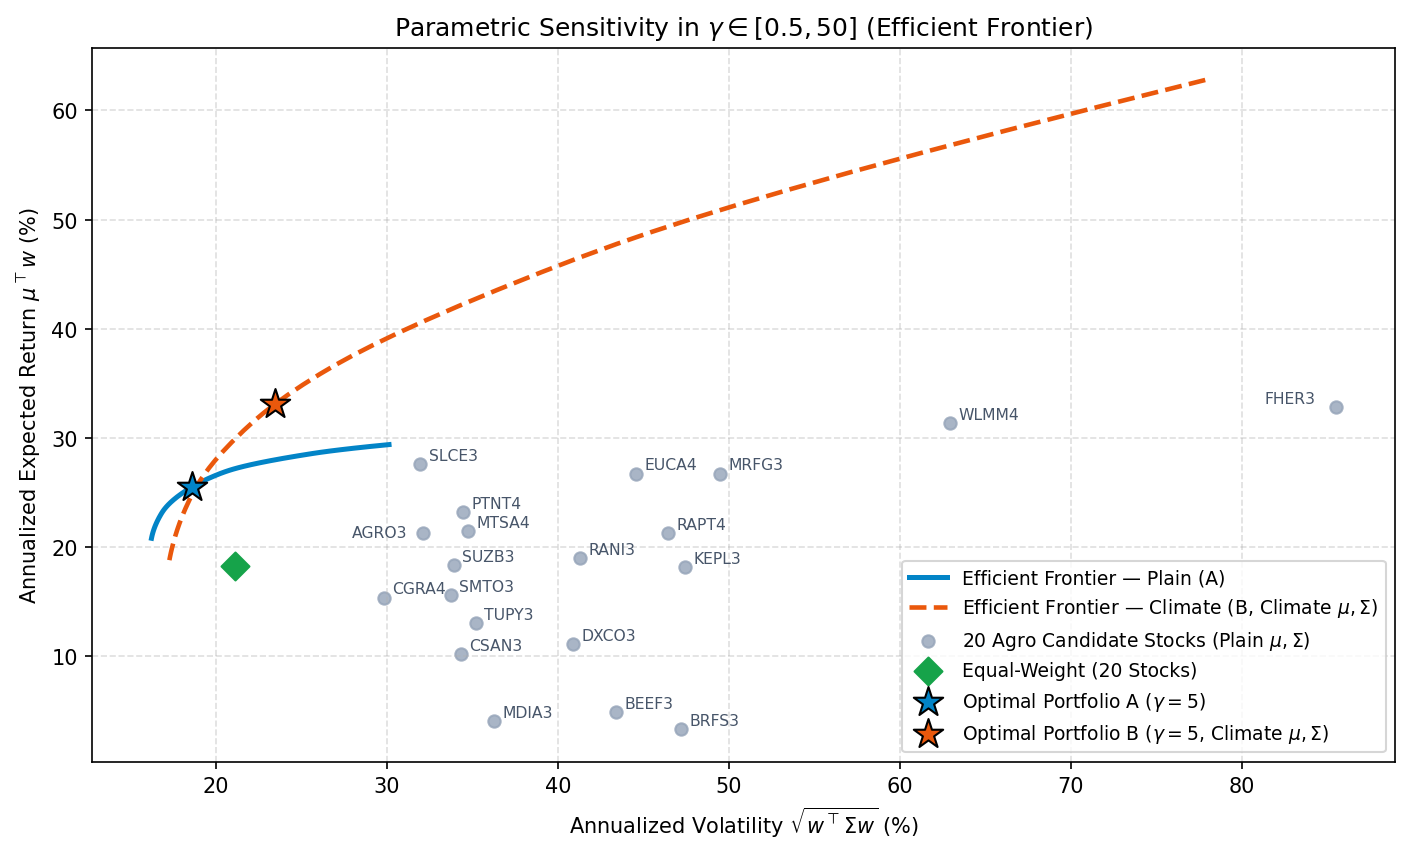
\includegraphics[width=\linewidth, height=0.65\textheight, keepaspectratio]{outputs/fig3_efficient_frontier.png}
      \end{figure}
    \end{column}
    \begin{column}{0.49\textwidth}
      \begin{figure}
        \centering
        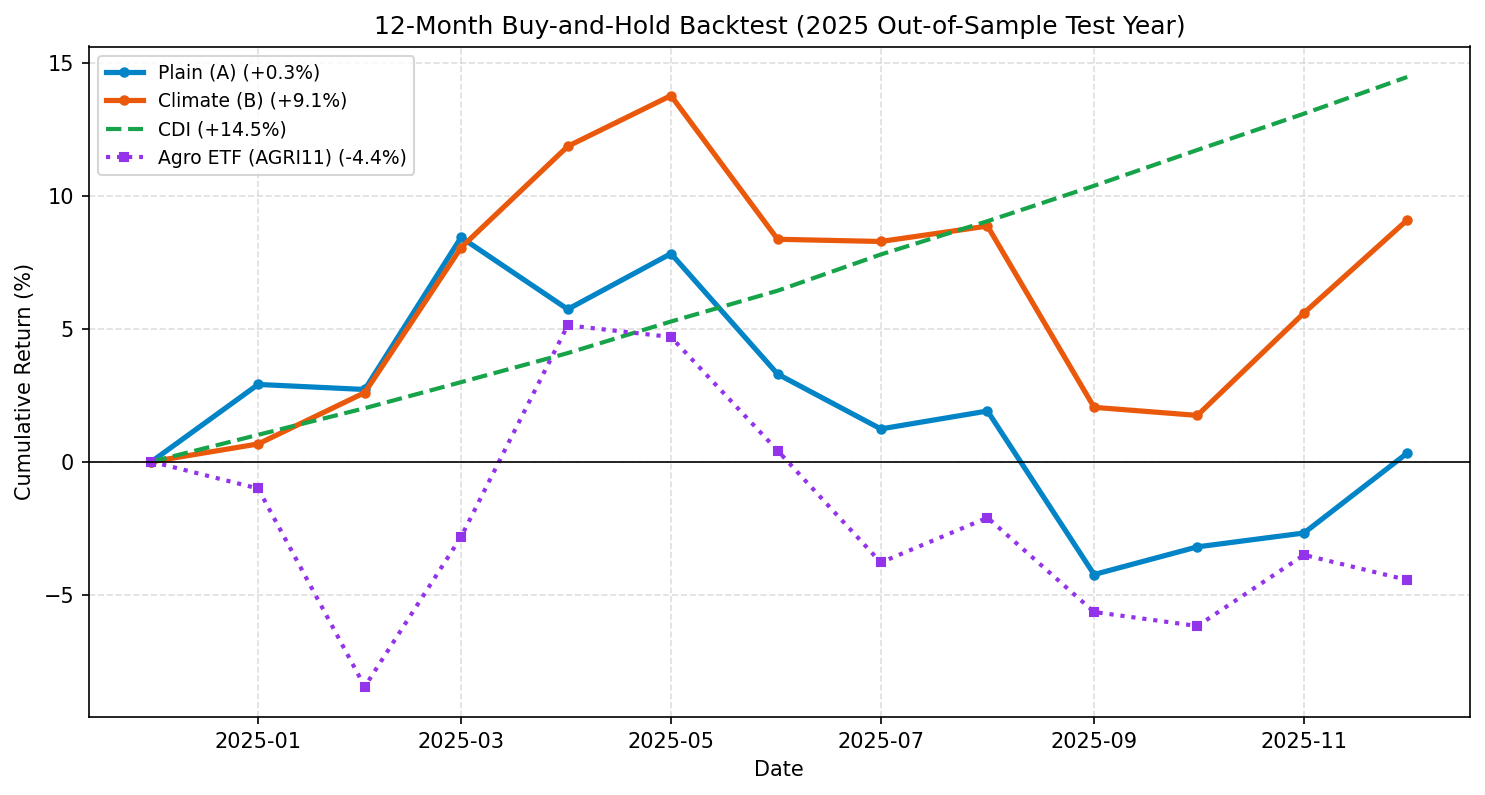
\includegraphics[width=\linewidth, height=0.65\textheight, keepaspectratio]{outputs/fig4_backtest_cumulative.png}
      \end{figure}
    \end{column}
  \end{columns}
  \vspace{0.1cm}
  \scriptsize
  \centering
  \textbf{2025 (12m buy-and-hold):} Clima $+9{,}08\%$ (Sharpe $-0{,}36$) $\mid$ Base $+0{,}32\%$ ($-1{,}11$) $\mid$ AGRI11 $-4{,}44\%$ ($-1{,}10$) $\mid$ CDI $+14{,}46\%$.
\end{frame}

%---------------------------------------------------------
% Slide 13: Limitações e Trabalhos Futuros
%---------------------------------------------------------
\begin{frame}{Limitações e Trabalhos Futuros}
  \textbf{Limitações:}
  \begin{itemize}
    \item Restrição exata de cardinalidade ($\|w\|_0 \le K$) exigiria variáveis binárias $z_i \in \{0,1\}$ (MIQP).
    \item Estimação estática de $(\mu, \Sigma)$ em janela fixa (2015--2024); erro de estimação de $\mu$ afeta o retorno realizado.
    \item Backtest de apenas 1 ano (2025) é ilustrativo da metodologia, não prova estatística de retorno.
  \end{itemize}

  \vspace{0.25cm}
  \textbf{Trabalhos Futuros:}
  \begin{itemize}
    \item Incorporar custos de transação (norma $\ell_1$) via métodos de pontos interiores ou gradiente proximal.
    \item Comparar com otimização robusta ou CVaR linearizado (PL/PLI).
  \end{itemize}
\end{frame}

%---------------------------------------------------------
% Slide 14: Referências
%---------------------------------------------------------
\begin{frame}{Referências}
  \scriptsize
  \begin{itemize}
    \item Markowitz, H. (1952). \emph{Portfolio Selection}. The Journal of Finance, 7(1), 77--91.
    \item Fiacco, A. V., \& McCormick, G. P. (1968). \emph{Nonlinear Programming: Sequential Unconstrained Minimization Techniques}. Wiley (SIAM, 1990).
    \item Karmarkar, N. (1984). \emph{A new polynomial-time algorithm for linear programming}. Combinatorica, 4(4), 373--395.
    \item Nesterov, Y., \& Nemirovski, A. (1994). \emph{Interior-Point Polynomial Algorithms in Convex Programming}. SIAM.
    \item Boyd, S., \& Vandenberghe, L. (2004). \emph{Convex Optimization}, Cap.~11 (Interior-Point Methods). Cambridge University Press.
  \end{itemize}
\end{frame}

%---------------------------------------------------------
% Slide 15: Obrigado
%---------------------------------------------------------
\begin{frame}
  \centering
  \Huge Obrigado!
\end{frame}

\end{document}
